\newcommand{\svcourse}{CST Part IA: Software Engineering and Security}
\newcommand{\svnumber}{1}
\newcommand{\svvenue}{Microsoft Teams}
\newcommand{\svdate}{2022-05-11}
\newcommand{\svtime}{15:00}
\newcommand{\svuploadkey}{CBd13xmL7PC1zqhNIoLdTiYUBnxZhzRAtJxv/ytRdM1r7qIfwMsxeVwM/pPcIo8l}

\newcommand{\svrname}{Dr Sam Ainsworth}
\newcommand{\jkfside}{oneside}
\newcommand{\jkfhanded}{yes}

\newcommand{\studentname}{Harry Langford}
\newcommand{\studentemail}{hjel2@cam.ac.uk}


\documentclass[10pt,\jkfside,a4paper]{article}

% DO NOT add \usepackage commands here.  Place any custom commands
% into your SV work files.  Anything in the template directory is
% likely to be overwritten!

\usepackage{fancyhdr}

\usepackage{lastpage}       % ``n of m'' page numbering
\usepackage{lscape}         % Makes landscape easier

\usepackage{verbatim}       % Verbatim blocks
\usepackage{listings}       % Source code listings
\usepackage{epsfig}         % Embed encapsulated postscript
\usepackage{array}          % Array environment
\usepackage{qrcode}         % QR codes
\usepackage{enumitem}       % Required by Tom Johnson's exam question header

\usepackage{hhline}         % Horizontal lines in tables
\usepackage{siunitx}        % Correct spacing of units
\usepackage{amsmath}        % American Mathematical Society
\usepackage{amssymb}        % Maths symbols
\usepackage{amsthm}         % Theorems

\usepackage{ifthen}         % Conditional processing in tex

\usepackage[top=3cm,
            bottom=3cm,
            inner=2cm,
            outer=5cm]{geometry}

% PDF metadata + URL formatting
\usepackage[
            pdfauthor={\studentname},
            pdftitle={\svcourse, SV \svnumber},
            pdfsubject={},
            pdfkeywords={9d2547b00aba40b58fa0378774f72ee6},
            pdfproducer={},
            pdfcreator={},
            hidelinks]{hyperref}


% DO NOT add \usepackage commands here.  Place any custom commands
% into your SV work files.  Anything in the template directory is
% likely to be overwritten!

\usepackage{fancyhdr}

\usepackage{lastpage}       % ``n of m'' page numbering
\usepackage{lscape}         % Makes landscape easier

\usepackage{verbatim}       % Verbatim blocks
\usepackage{listings}       % Source code listings
\usepackage{graphicx}
\usepackage{float}
\usepackage{epsfig}         % Embed encapsulated postscript
\usepackage{array}          % Array environment
\usepackage{qrcode}         % QR codes
\usepackage{enumitem}       % Required by Tom Johnson's exam question header

\usepackage{hhline}         % Horizontal lines in tables
\usepackage{siunitx}        % Correct spacing of units
\usepackage{amsmath}        % American Mathematical Society
\usepackage{amssymb}        % Maths symbols
\usepackage{amsthm}         % Theorems

\usepackage{ifthen}         % Conditional processing in tex

\usepackage[top=3cm,
            bottom=3cm,
            inner=2cm,
            outer=5cm]{geometry}

% PDF metadata + URL formatting
\usepackage[
            pdfauthor={\studentname},
            pdftitle={\svcourse, SV \svnumber},
            pdfsubject={},
            pdfkeywords={9d2547b00aba40b58fa0378774f72ee6},
            pdfproducer={},
            pdfcreator={},
            hidelinks]{hyperref}

\renewcommand{\headrulewidth}{0.4pt}
\renewcommand{\footrulewidth}{0.4pt}
\fancyheadoffset[LO,LE,RO,RE]{0pt}
\fancyfootoffset[LO,LE,RO,RE]{0pt}
\pagestyle{fancy}
\fancyhead{}
\fancyhead[LO,RE]{{\bfseries \studentname}\\\studentemail}
\fancyhead[RO,LE]{{\bfseries \svcourse, SV~\svnumber}\\\svdate\ \svtime, \svvenue}
\fancyfoot{}
\fancyfoot[LO,RE]{For: \svrname}
\fancyfoot[RO,LE]{\today\hspace{1cm}\thepage\ / \pageref{LastPage}}
\fancyfoot[C]{\qrcode[height=0.8cm]{\svuploadkey}}
\setlength{\headheight}{22.55pt}


\ifthenelse{\equal{\jkfside}{oneside}}{

 \ifthenelse{\equal{\jkfhanded}{left}}{
  % 1. Left-handed marker, one-sided printing or e-marking, use oneside and...
  \evensidemargin=\oddsidemargin
  \oddsidemargin=73pt
  \setlength{\marginparwidth}{111pt}
  \setlength{\marginparsep}{-\marginparsep}
  \addtolength{\marginparsep}{-\textwidth}
  \addtolength{\marginparsep}{-\marginparwidth}
 }{
  % 2. Right-handed marker, one-sided printing or e-marking, use oneside.
  \setlength{\marginparwidth}{111pt}
 }

}{
 % 3. Alternating margins, two-sided printing, use twoside.
}


\setlength{\parindent}{0em}
\addtolength{\parskip}{1ex}

% Exam question headings, labels and sensible layout (courtesy of Tom Johnson)
\setlist{parsep=\parskip, listparindent=\parindent}
\newcommand{\examhead}[3]{\section{#1 Paper #2 Question #3}}
\newenvironment{examquestion}[3]{
\examhead{#1}{#2}{#3}\setlist[enumerate, 1]{label=(\alph*)}\setlist[enumerate, 2]{label=(\roman*)}
\marginpar{\href{https://www.cl.cam.ac.uk/teaching/exams/pastpapers/y#1p#2q#3.pdf}{\qrcode{https://www.cl.cam.ac.uk/teaching/exams/pastpapers/y#1p#2q#3.pdf}}}
\marginpar{\footnotesize \href{https://www.cl.cam.ac.uk/teaching/exams/pastpapers/y#1p#2q#3.pdf}{https://www.cl.cam.ac.uk/\\teaching/exams/pastpapers/\\y#1p#2q#3.pdf}}
}{}


\usepackage{listings}
\usepackage{tikz}

\lstdefinestyle{cstyle}{
  belowcaptionskip=1\baselineskip,
  breaklines=true,
  xleftmargin=\parindent,
  language=C,
  showstringspaces=false,
  basicstyle=\footnotesize\ttfamily,
  keywordstyle=\bfseries\color{orange!80!black},
  commentstyle=\itshape\color{purple!40!black},
  identifierstyle=\color{blue},
  stringstyle=\color{green!40!black},
}

\lstdefinestyle{pseudocode}{
  belowcaptionskip=1\baselineskip,
  breaklines=true,
  xleftmargin=\parindent,
  language=C,
  showstringspaces=false,
  basicstyle=\footnotesize\ttfamily,
  keywordstyle=\bfseries\color{orange!80!black},
  commentstyle=\itshape\color{purple!40!black},
  stringstyle=\color{green!40!black},
}


\begin{document}

\begin{examquestion}{2015}{2}{3}

\begin{enumerate}

\item What is an access control list?

An access control list is a list of users and their priviliges for a specific file.
The access control list is associated with each file allowing maximum flexibility. 
There are three priviliges:
read, write and execute -- each of which have a single bit. This allows different users to 
have different priviliges for the same file.

Initially on all accesses of files, the process trying to access does not have priviliges. 
This causes a segment fault. 
At this point we load in the access-control-list and check to see whether the process should 
have access. If it should then 
access is granted and if it should not then the process is terminated. Access can be granted 
or elevated only by the owner.

\item What is a capability in the context of access control?

Capabilities are unique and unforgeable identifiers for files. If a process has it then the 
file knows 
that it should have the access granted by this capability. However, capabilities can be 
passed to other processes. This leaves the possibility of processes having access that 
they were not directly granted. Capabilities and what accesses they should give are stored 
in the files 
inode. This means that the priviliges they give can be rapidly updated.

\item How is file access control in Unix implemented, and what simplifications are
made over one of the general mechanisms you have described above?

UNIX uses access-control-lists. However, rather than giving access rights to users, it gives 
access rights to groups of users. This means that on large systems we do not have large amounts 
of duplicate data across files. There are three categories: owner, group and universe. 
The owner has full access rights to the file. Groups have whatever access rights the owner 
has assigned to their group. The universe is anyone who's not the owner and is not in a group. 
The universe typically has the lowest access level. Each file grants rights to the owner, one 
group and the universe. For each category there are three bits: Read, Write and Execute (RWX). 
This means that a fixed amount of bits are needed for each access control list, greatly simplifying 
the system: holding variable-length access-control lists for each system would make memory management 
much more complicated -- variable length inodes. Some systems support more than one group -- as long 
as the number of groups supported is less than a constant the system will work. Note that there are 
only 8 possible combinations of access and so having more than 8 groups per file makes no sense. 
Groups can be stored on other pages. So groups only need to be listed once. This decreases 
the amount of duplicate data and saves space.

Note that UNIX does not use capabilities: but Linux does.

\item What is the principle of minimum privilege and which approach, access control
lists or capabilities, lends itself better to supporting a minimum privilege regime?

The principle of minimum privilige means you give each process the minimum privilige 
that it needs to do whatever it should do. This way the process is physically unable to 
do most of the things it should not be able to do and if it tries to do them, it will 
raise a semgent fault -- which can be dealt with accordingly.

Access Control Lists support the principle of minimum privilige better than capabilities.

The main reason for this is that capabilities are held by programs and can be passed around, 
if one rogue program gets a capability then the whole system can have the same capability even 
if it they were not directly given the capability. This is not the same with access control lists. 

Since capabilities risk ``leaking'' access to files, I believe that access-control-lists better 
conform to the principle of minimum privilige.

\end{enumerate}

\end{examquestion}

\begin{examquestion}{2014}{2}{3}

One goal of a multiuser operating system is to protect each user’s information and
activity from damage caused by accidental or deliberate actions of other users of the
system.

\begin{enumerate}

\item \label{prempt} Describe a mechanism that operating systems use to reduce the opportunity for
a user process to prevent another user’s process from making progress. In your
description include any particular hardware features that are relied upon.

Pre-emptive scheduling will interrupt every process eventually. A good pre-emptive scheduler 
will assign the process which has just been moved from the running state to the ready 
state a lower priority. This prevents denial of service. Pre-emptive scheduling relies 
upon hardware support for context switches.

\item \label{alternatives} Describe two alternative mechanisms that operating systems could use to reduce
the opportunity for a user process to access or corrupt the information being used
by another user’s process. In your descriptions include any particular hardware
features that are relied upon.

If we use virtual addressing then processes are physically incapable of accessing 
other processes address spaces. This relies upon hardware support for traversing 
page tables and hardware support for converting virtual addresses to physical addresses.

We must also empty the TLB after context-switching processes. This 
relies on hardware support from the TLB to rapidly remove all data.

\item \label{longterm} Describe how an operating system might attempt to ensure that long-term user
information (that is, information which exists beyond process execution) is not
interfered with or misused by other users. Your description should be clear
about when actions are performed and the resources they consume.

We can give files access rights to ensure that long term information is not 
interfered with. Each file should have an owner, group and universe access rights. 
These can be chosen so that users files give full access to the users processes and 
restricted access to other users processes. For example giving the owner RWX (read-write-execute), 
giving no groups access and giving the universe no access.

When a process tries to access a new file, it will cause a segment fault (since the process 
has not been granted access -- although it may have sufficient priviliges). At this point, the 
CPU can check the access bits to see whether the process trying to access the file has sufficient 
priviliges. If it does then access is granted and tha page is loaded into memory. 

\item To what extent are the mechanisms described above useful in single user
systems?

The mechanisms described above are still useful in single user systems. The difference 
is that now rather than preventing different users corrupting other users files 
we are preventing processes corrupting processes being run by the same user and preventing 
processes occupying all the CPU time. The measures described in part \ref{prempt} will ensure 
that tasks cannot deny service to other processes.

If we did not have \ref{prempt} then the below code would loop infinitely and prevent all 
other programs from running.
\begin{lstlisting}[style=cstyle]
void main()
{
	start:
	goto start;
}
\end{lstlisting}


Virtual memory (discussed in \ref{alternatives}) is still necessary since we do not 
want processes to interfere with other processes address space irrelevant of whether the 
other process belongs to another user or not. An analagous argument can be made 
regarding flushing the TLB.

Access rights are still relevant in a single-user system. You do not with every process 
to have full read-write-execute access on all programs.

\item How do operating systems ensure that they are not themselves overly-restricted
by these mechanisms?

The Operating System is a high priority task and so is not interrupted by the scheduler 
when running. The Operating System does not need to read-write or execute user-files 
and so the permissions for those are not relevant and will not restrict the Operating System. 

We have high hardware support for all of these processes. This means that execution is not 
slowed down significantly.

\end{enumerate}

\end{examquestion}

\begin{examquestion}{2011}{2}{4}

\begin{enumerate}

\item In the context of memory management:

\begin{enumerate}

\item What is the address binding problem?

The problem of deciding \textit{where} the physical addresses of variables in 
programs should be.

\item  The address binding problem can be solved at compile time, load time or
run time. For each case, explain what form the solution takes, and give
one advantage and one disadvantage.

Program $C$:
\begin{lstlisting}[style=cstyle]
#include <stdio.h>

void main()
{
	int i = 0;
	scanf("%d", &i);
	if (i == 0)
	{
		int j = 1;
		int k = 2;
		int l = 3;
	}
}
\end{lstlisting}

\begin{itemize}

\item If we decide where to allocate memory at compile time, then we can run 
algorithms determining the optimal place to allocate it. This means that 
our program will be faster than other methods (although the compile time is 
far longer). Note also that we only run this algorithm once. 

However, if we decide where to allocate memory at compile time then we have to allocate 
all the memory the program \textit{might} need throughout execution. This is necessary 
even if the program never uses some of these variables; so if we allocated memory 
at compile time, when running program $C$, we would 
allocate memory for $j$, $k$ and $l$ even if $i \neq 0$ at execution.
If we decide where to allocate memory at compile time then we have to use absolute 
addresses. This is impractical in general purpose systems: we will not be able to run two 
programs which expect to use the same absolute addresses.

\item If we allocate memory at load-time then we do not suffer from ``processes expecting to 
use the same addresses''. 

However, we must parse through the whole program and 
decide where we should place every variable which could exist in the program. This is 
very expensive and a large overhead before running any program. While we can run algorithms 
to make memory locations chosen more optimal, this has to be done every call.
If we ran Program $C$, note we would still have to allocate memory for $j$, $k$, $l$.

\item Allocating memory at runtime means we do not have to allocate any memory 
unless we use it. If we ran program $C$, then we would not have to allocate memory 
for $j$, $k$ or $l$. With hardware support, we can automatically translate between program 
addresses and real addresses. This means that we do not have to change the addresses 
in the program itself at runtime. 

This scheme also does not suffer from ``multiple programs 
expecting to use the same memory'' either and we cna dynamically allocate more memory 
when needed. However we cannot run advanced optimisation algorithms to choose the best 
location for the memory addresses.

\end{itemize}

\item Under which circumstances do external and internal fragmentation occur?
How can each be handled?

External fragmentation happens when placing data of different sizes straight into memory. 
An example of this is segmentation -- where many different sized data leave many small 
gaps between them which are too small to be used. This can be lessened by using a 
heuristic method of choosing where to put data: ie best-fit or worst-fit. External 
fragmentation can be handled by compaction: moving data around in memory to make the 
spaces contiguous.

Internal fragmentation is caused by placing data of many sizes into uniformly sized blocks of 
data. Some of these blocks will be too large for the data placed inside them rendering 
part of the block unusable. This can be handled by using smaller blocks. Although using 
smaller blocks means more memory accesses: there is a trade-off.

\item What is the purpose of a translation lookaside buffer (TLB)?

Caching pages:

Memory accesses are long and slow while the TLB is far faster to read from. TLB's have 
expensive and fast hardware so that searching the TLB is significantly faster than 
searching memory. Modern TLB's can have a 98\% hit rate -- meaning that 98\% of pages we 
try to find will be in the TLB. This dramatically speeds up memory accesses.

\end{enumerate}

\item Describe how UNIX handles user authentication.

On startup, you load the kernel from disk and start executing it. This then 
runs the login program. This copies some programs and forks some stuff. Each 
process then outputs login and waits for the user to input their username. 
It then takes a password and checks whether it hashes to the same value as the 
password stored on disk.

\end{enumerate}

\end{examquestion}

\begin{examquestion}{2009}{2}{3}

\begin{enumerate}\setcounter{enumi}{1}

\item In the context of the UNIX operating system:

\begin{enumerate}

\item What is a pipe? What is it used for? How does it operate? Use a diagram
to illustrate your answer.

An ordinary pipe is a special type of FIFO file which parent processes share 
with child processes. This allows the parent to write into one end of the pipe and 
the child to read from the other end of the pipe. This is a very basic type of 
inter-process communication. Note that unnamed pipes are unidirectional: the parent 
can send data to the child \textit{or} the child can send data to the parent. To achieve 
bidirectional data transmission we simply use two pipes.

\begin{center}
\begin{tikzpicture}
\node (write) [anchor=center] at (-1, 0) {write};
\node (read) [anchor=center] at (4, -1) {read};
\node (pipe) [anchor=south] at (1.5, 0) {pipe};
\draw [fill=lightgray] (0, 0) rectangle (3, -1);
\draw [fill=white] (0, 0) rectangle (0.3, -1);
\draw [fill=white] (0.3, 0) rectangle (0.6, -1);
\draw [fill=green!80!black] (0.6, 0) rectangle (0.9, -1);
\draw [fill=green!80!black] (0.9, 0) rectangle (1.2, -1);
\draw [fill=green!80!black] (1.2, 0) rectangle (1.5, -1);
\draw [fill=green!80!black] (1.5, 0) rectangle (1.8, -1);
\draw [fill=green!80!black] (1.8, 0) rectangle (2.1, -1);
\draw [fill=lightgray] (2.1, 0) rectangle (2.4, -1);
\draw [fill=lightgray] (2.4, 0) rectangle (2.7, -1);
\draw [fill=lightgray] (2.7, 0) rectangle (3.0, -1);
\node (left) at (0.6, -0.5) {};
\node (right) at (1.8, -0.5) {};
\draw [thick] (0, 0) -- (3, 0);
\draw [thick] (0, -1) -- (3, -1);
\draw [-stealth] (write) to [out=270, in=180] (left);
\draw [-stealth] (right) to [out=0, in=90] (read);
\node (free) [anchor=center] at (0.3, -1.8) {free space};
\node (new) [anchor=center] at (1.35, -2.5) {new data};
\node (old) [anchor=center] at (2.55, -1.8) {old data};
\node (A) [anchor=center] at (-2, -0.5) {Parent};
\node (B) [anchor=center] at (5, -0.5) {Child};
\draw [-stealth] (0.15, -0.9) to [out=270, in=90] (free);
\draw [-stealth] (0.45, -0.9) to [out=270, in=90] (free);
\draw [-stealth] (0.75, -0.9) to [out=270, in=90] (new);
\draw [-stealth] (1.05, -0.9) to [out=270, in=90] (new);
\draw [-stealth] (1.35, -0.9) to [out=270, in=90] (new);
\draw [-stealth] (1.65, -0.9) to [out=270, in=90] (new);
\draw [-stealth] (1.95, -0.9) to [out=270, in=90] (new);
\draw [-stealth] (2.25, -0.9) to [out=270, in=90] (old);
\draw [-stealth] (2.55, -0.9) to [out=270, in=90] (old);
\draw [-stealth] (2.85, -0.9) to [out=270, in=90] (old);
\end{tikzpicture}
\end{center}

Note there is another type of pipe: named pipes (FIFO's in UNIX).\\
Named pipes are also FIFO files -- 
except they are bidirectional; they can be written to and read from by many different 
processes without parent-child dependencies; and they are persistent: 
name pipes are not automatically deleted after the processes stop communicating -- 
they must be explicitly deleted.

\item  What is the shell? Describe its operation in pseudo-code, giving special
emphasis to any system calls invoked.

A shell is a command interpreter. It is a program which allows users to manipulate the 
file store, read from and write to and execute files. Shells allow users to use relative 
paths. This makes manipulation of the file system easier.

Here is pseudo-code describing what a shell does:

\begin{lstlisting}[style=pseudocode]
#include <all>
/*
this is not an actual library: rather it signifies that we should 
include all libraries in the path and builtin libraries etc.
In a real system many of these would be loaded when called 
to be more efficient -- however the effect is the same.
*/

void main()
{
	string instruction;
	function(string[]) command;
	string[] args;
	bool successful;
	interpreter:
	printf(">");
	scanf("%s", &instruction);
	command = get_function_to_execute(instruction);
	if (command == NULL)
	{
		printf("No such command");
		goto interpreter;
	}
	args = get_arguments(instruction);
	if (fork() == 0){
		execve(command, args);
		exit();
	}
	goto interpreter;
}
\end{lstlisting}

\end{enumerate}

\end{enumerate}

\end{examquestion}

\end{document}